\documentclass[10pt]{exam}
\usepackage[icp]{template-for-exam}
\usepackage{tikz,multicol,enumitem}


\title{Post-Break Chemistry Review}
\author{Rohrbach}
\date{\today}

\begin{document}
\maketitle

\newcommand{\ptable}{
  \begin{center}
    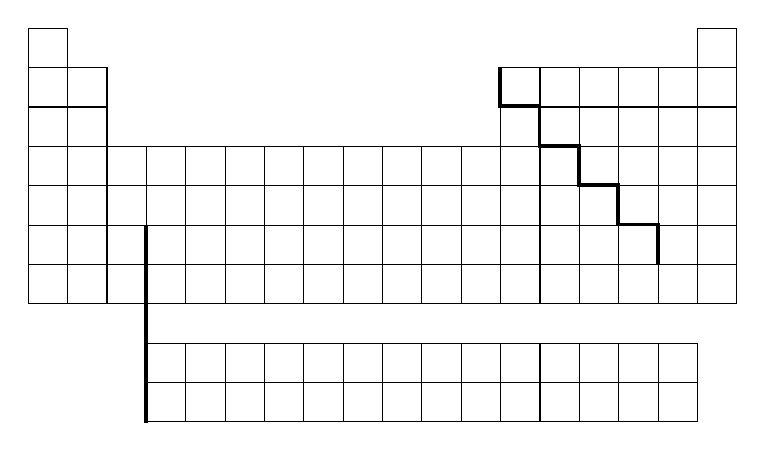
\begin{tikzpicture}
      \def\elsize{0.5cm}
      \tikzstyle{e} = [
        minimum width=\elsize, 
        minimum height=\elsize, 
        node distance=\elsize,
        draw=black
      ]
  
      \node[e, anchor=north west] at (0,0) (1) {};
  
      \node[e,below of=1] (1) {};
      \node[e,right of=1] (2) {};
  
      \node[e,below of=1] (1) {};
      \node[e,right of=1] (2) {};
  
      \node[e,below of=1] (1) {};
      \foreach \x in {1,...,17} {
        \pgfmathtruncatemacro{\y}{\x+1}
        \node[e, right of=\x] (\y) {};
      }
  
      \node[e, above of=13] (13) {};
      \foreach \x in {13,...,17} {
        \pgfmathtruncatemacro{\y}{\x+1}
        \node[e, right of=\x] (\y) {};
      }
  
      \node[e, above of=13] (13) {};
      \foreach \x in {13,...,17} {
        \pgfmathtruncatemacro{\y}{\x+1}
        \node[e, right of=\x] (\y) {};
      }
  
      \node[e, above of=18] (18) {};
  
      \foreach \per in {4,5,6} {
        \node[e, below of=1] (1) {};
        \foreach \x in {1,...,17} {
          \pgfmathtruncatemacro{\y}{\x+1}
          \node[e, right of=\x] (\y) {};
        }
      }
  
      \node[e, below of=4,node distance=2*\elsize] (4) {};
      \foreach \x in {4,...,16} {
        \pgfmathtruncatemacro{\y}{\x+1}
        \node[e, right of=\x] (\y) {};
      }
      \node[e, below of=4] (4) {};
      \foreach \x in {4,...,16} {
        \pgfmathtruncatemacro{\y}{\x+1}
        \node[e, right of=\x] (\y) {};
      }
  
      \draw[line width=.5mm] (12*\elsize,-\elsize) 
        -- ++(0,-\elsize)
        -- ++(\elsize,0)
        -- ++(0,-\elsize)
        -- ++(\elsize,0)
        -- ++(0,-\elsize)
        -- ++(\elsize,0)
        -- ++(0,-\elsize)
        -- ++(\elsize,0)
        -- ++(0,-\elsize);


      \draw[line width=0.5mm] (3*\elsize,-5*\elsize) 
        -- ++(0,-5*\elsize)
        -- ++(0,-0.15mm);
      
    \end{tikzpicture}
  \end{center}
}


\begin{questions}
  \question  Shade in the {\bf metals} on the periodic table: \ptable
  \question  Shade in the {\bf nonmetals} on the periodic table: \ptable
  \question  Draw dot diagrams for the following elements:
    \begin{multicols}{2}
      \begin{parts}
        \part Lithium \vspace{2em}
        \part Antimony \vspace{2em}
        \part Aluminum \vspace{2em}
        \part Chlorine \vspace{2em}
        \part Neon \vspace{2em}
        \part Beryllium \vspace{2em}
        \part Germanium \vspace{2em}
        \part Oxygen \vspace{2em}
  
      \end{parts}
    \end{multicols}
  \question Explain the {\bf ``octet rule''} for elements \vs
  \pagebreak
  \question Fill in this table:

  \renewcommand{\arraystretch}{4}

  \begin{center}
    \begin{tabular}{|l|l|l|l|p{5em}|p{5em}|}
    \hline
    Element & Dot Diagram & Gain or lose? & How many? & Charge & Symbol \\\hline
    Sodium & & & & & \\\hline
    Chlorine & & & & & \\\hline
    Neon & & & & & \\\hline
    Strontium & & & & & \\\hline
    \end{tabular}
    \end{center}
\end{questions}

\end{document}